\documentclass[a4paper, 12pt]{article}
\usepackage{graphicx} % Required for inserting images
\usepackage{fullpage}
\usepackage{amsmath}
\usepackage[dvipsnames]{xcolor}
\usepackage{float}
\usepackage{geometry}
\usepackage{biblatex}
\geometry{margin=1in}
\usepackage{enumitem}
\usepackage{parskip}
\usepackage{pgfplots}
\pgfplotsset{compat=1.18}
\usepackage[normalem]{ulem}
\usepackage[version=4]{mhchem}
\usepackage{tikz}
\usepackage{microtype}
\usepackage{gensymb}
\usepackage{caption}
\usepackage{cancel}
\usepackage{nicefrac}

\newcommand{\degC}{$\degree$C \,}
\newcommand{\degF}{$\degree$F \,}
\newcommand{\R}{\left(0.0821 \: \frac{L \cdot atm}{mol \cdot \text{K}}\right)}
\newcommand{\cunits}{$\frac{J}{g \degree \text{C}}$}
\newcommand{\Hf}{$\Delta H_\text{f}$} % heat of formation
\newcommand{\mathHf}{\Delta H_\text{f}} %heat of formation in math mode

\usepackage{hyperref}
\hypersetup{
colorlinks = true,
linkcolor = teal,
citecolor=teal,         % Set color for citations
filecolor=teal,         % Set color for file links
urlcolor=teal           % Set color for URLs
}

\title{Chemistry Honors Study Guide}
\author{Semester 2 Final Exam}
\date{Test date: the calendar is glitching help}

\begin{document}

\maketitle

\tableofcontents

\newpage

\section{Limiting and Excess Reagents}

\subsection{Definitions}

\begin{itemize}[leftmargin=*, nosep]
    \item \textbf{\textit{limiting (lim) reagent:}} The reactant that limits the amount of product yielded to a certain number.
    \item \textbf{\textit{excess (xs) reagent:}} The reactant left over after all of the limiting reagent is used.
    \item \textbf{\textit{theoretical yield:}} The theoretical amount of product produced found through calculations.
    \item \textbf{\textit{actual yield:}} The amount of product actually produced, likely affected by sources of error, found by doing the experiment. (Also \textit{experimental yield.})
    \item \textbf{\textit{percent yield:}} The percentage of the theoretical yield that is actually produced through experimentation.
\end{itemize}

\subsection{Finding Limiting Reagent and Theoretical Yield}
A limiting reagent limits the amount of product that can be created in a chemical reaction (no matter how much of the other reactant you have, the limiting reagent controls the maximum reactant produced, known as theoretical yield).

Example:

$$2\text{HCl} + \text{Zn} \longrightarrow \text{ZnCl}_2 + \text{H}_2$$

If you react \textcolor{blue}{17 $g$ HCl} with \textcolor{blue}{17 $g$ Zn}, what is the limiting reagent and theoretical yield of ZnCl$_2$?

\textcolor{blue}{\textbf{Step 1:} Find how many grams of ZnCl$_2$} each reactant provides.

$$(17 \: g \: \text{HCl}) \times \left(\frac{1 \: mol \: \text{HCl}}{36.461 \: g \: \text{HCl}}\right) \times \left(\frac{1 \: mol \: \text{ZnCl}_2}{2 \: mol \: \text{HCl}}\right) \times \left(\frac{136.286 \: g \: \text{ZnCl}_2}{1 \: mol \: \text{ZnCl}_2}\right)$$

$$ \approx 31.77 \: g \: \text{ZnCl}_2$$

$$(17 \: g \: \text{Zn}) \times \left(\frac{1 \: mol \: \text{Zn}}{65.38 \: g \: \text{Zn}}\right) \times \left(\frac{1 \: mol \: \text{ZnCl}_2}{1 \: mol \: \text{Zn}}\right) \times \left(\frac{136.286 \: g \: \text{ZnCl}_2}{1 \: mol \: \text{ZnCl}_2}\right)$$

$$ \approx 35.44 \: g \: \text{ZnCl}_2$$

\textcolor{blue}{\textbf{Step 2:} Find the limiting reagent} by taking the element that produces the smallest amount of the product (the theoretical yield). The excess reagent is the other reactant.

\fbox{
\begin{minipage}{0.4\textwidth} 
limiting reagent: HCl \\ 
excess reagent: Zn \\ 
theoretical yield: 31.77 g ZnCl$_2$ 
\end{minipage}}

\subsection{Finding Percent Yield}
To find the percent yield, use this formula:

$$\frac{\text{actual yield}}{\text{theoretical yield}} \times 100\%$$

\subsection{Finding Amount of Excess Reagent}
To find the amount of excess reagent left over after a reaction has occurred, work backwards from the theoretical yield.

Example:

$$\text{Al} + \text{MgCl}_2 \longrightarrow \text{AlCl}_3 + \text{Mg}$$

If you react \textcolor{blue}{10 $g$ Al} with \textcolor{blue}{10 $g$ MgCl$_2$}, how many grams of excess reagent are there?

\textcolor{blue}{\textbf{Step 1:} Always check if the equation is balanced}, and if not, balance it.

$$\text{2Al} + \text{3MgCl}_2 \longrightarrow \text{2AlCl}_3 + \text{3Mg}$$

\textcolor{blue}{\textbf{Step 2:} Find the theoretical yield} by applying the steps shown in the prior example.

$$(10 \: g \: \text{Al}) \times \left(\frac{1 \: mol \: \text{Al}}{26.982 \: g \: \text{Al}}\right) \times \left(\frac{2 \: mol \: \text{AlCl}_3}{2 \: mol \: \text{Al}}\right) \times \left(\frac{133.341 \: g \: \text{AlCl}_3}{1 \: mol \: \text{AlCl}_3}\right)$$

$$ \approx 49.42 \: g \: \text{AlCl}_3$$

$$(10 \: g \: \text{MgCl}_2) \times \left(\frac{1 \: mol \: \text{MgCl}_2}{95.211 \: g \: \text{MgCl}_2}\right) \times \left(\frac{2 \: mol \: \text{AlCl}_3}{3 \: mol \: \text{MgCl}_2}\right) \times \left(\frac{133.341 \: g \: \text{AlCl}_3}{1 \: mol \: \text{AlCl}_3}\right)$$

$$ \approx 9.34 \: g \: \text{AlCl}_3 \longleftarrow \text{\textcolor{red}{theoretical yield, lim. reagent is MgCl$_2$}}$$

\textcolor{blue}{\textbf{Step 3:} Work backwards from the theoretical yield} and find how many grams of excess reagent (Al) is needed to produce approximately 9.3 grams of AlCl$_3$.

$$(9.3 \: g \: \text{AlCl}_3) \times \left(\frac{1 \: mol \: \text{AlCl}_3}{133.341 \: g \: \text{AlCl}_3}\right) \times \left(\frac{2 \: mol \: \text{Al}}{2 \: mol \: \text{AlCl}_3}\right) \times \left(\frac{26.982 \: g \: \text{Al}}{1 \: mol \: \text{Al}}\right)$$

$$\approx 1.88 \: g \: \text{Al}$$

\textcolor{blue}{\textbf{Step 4:} Subtract this number} from the amount of aluminum used in the reaction to get $10 - 1.88 = \boxed{8.12 \: g}$ of excess reagent.

\textcolor{blue}{\textbf{Step 5:} Check if the answer is reasonable.} There was a large difference between the product yielded by the magnesium chloride and the aluminum, so it makes sense that there is a significant amount of aluminum left over.

\section{Ionic Reactions}

\subsection{Types of Reactions} \label{types of reactions}

\paragraph{Combination reaction}
Two or more reactants combine to create one product
$$ A + B \longrightarrow AB$$

\paragraph{Decomposition reaction}
Reactant decomposes into two or more products
$$ AB \longrightarrow A + B$$ 

\paragraph{Double displacement reaction}
Two ionic compounds switch anions
$$ AB + CD \longrightarrow AD + CB$$ 

\paragraph{Single displacement reaction}
The anion switches from one reactant to the other (note: when predicting products, diatomic elements that stand alone should have 2 as a subscript)
$$ A + BC \longrightarrow AC + B$$ 

\paragraph{Combustion reaction}
Substance reacts with oxygen, creating energy (heat)
$$ \text{C}_x\text{H}_y + \text{O}_2 \longrightarrow \text{H}_2\text{O} + \text{CO}_2$$

\paragraph{Neutralization reaction}
An acid reacts with a base to form water and an ionic compound

$$\text{H}A + B\text{OH} \longrightarrow \text{H$_2$O +} BA $$

\subsection{Ionic Equations}

\textbf{Balanced chemical eqn. (B.C.E.) or molecular equation}

$$2\text{AgNO}_{3(aq)} + \text{CuCl}_{2(aq)} \longrightarrow 2\text{AgCl}_{(s)} + \text{Cu(NO$_3$)}_{2(aq)}$$

\textbf{(Overall) ionic eqn. (I.E.):} break apart aq. compounds (bring subscript to the front)

$$2\text{Ag}^+ + 2{\text{NO}_3}^- + \text{Cu}^{2+} + 2\text{Cl}^- \longrightarrow 2\text{AgCl} + \text{Cu}^{2+} + {2\text{NO}_3}^-$$

(do not need subscripts)

Compounds that can be cancelled out (\textbf{spectator ions}) are not involved in the reaction. ($2\text{NO}_3^-$ and $\text{Cu}^{2+}$)

\textbf{Net ionic eqn. (N.I.E.):} get rid of compounds that cancel out (should be charge-balanced)

$$2\text{Ag}^+ + 2\text{Cl}^- \longrightarrow 2\text{AgCl}$$

This is the actual reaction that occurs.

\textcolor{red}{No net ionic equation, all spectator ions, all aqueous = NO REACTION}

\textbf{Precipitation rxn w/ ppt (precipitate, $(s)$)}

$$(aq) + (aq) \longrightarrow (s) + (aq)$$

\subsection{Solubility Rules} \label{solubility rules}
These rules are provided on tests and quizzes and do not need to be memorized. Soluble = aqueous, insoluble = solid.

\begin{enumerate}[leftmargin=*, nosep]
    \item Alkali metals (group 1) are always soluble.
    \item Ammonium, (NH$_4$$^+$) is always soluble.
    \item Nitrates (NO$_3$$^-$), chlorates (Cl$_3$$^-$), and perchlorates (ClO$_4$$^-$)
    \item Most hydroxides (OH$^-$) are insoluble except those paired with an alkali metal or barium.
    \item Most chlorides (Cl$^-$), bromides (Br$^-$), and iodides chlorides (I$^-$) are soluble except when they are paired with silver (Ag$^+$), lead (Pb$^{2+}$), and mercury (Hg$^{2+}$).
    \item Carbonates (CO$_2$$^{3-}$), phosphates (PO$_4$$^{3-}$), and sulfides (S$^{2-}$) are insoluble except when paired with ammonium (NH$_4$$^+$) and alkali metals.
    \item Most sulfates (SO$_4$$^{2-}$) are soluble except barium sulfate (BaSO$_4$), lead sulfate (PbSO$_4$), and mercury sulfate (HgSO$_4$).
\end{enumerate}

\section{Solutions}

\subsection{Definitions}

\begin{itemize}[leftmargin=*, nosep]
    \item \textbf{\textit{solution:}} A homogeneous mixture in the liquid phase.
    \item \textbf{\textit{solvent:}} The larger part of the solution in the liquid phase.
    \item \textbf{\textit{solute:}} The smaller part of the solution that is dissolved in the solvent. Can be solid, liquid, or gas.
    \item \textbf{\textit{percent by mass:}} The percentage of the solution that is the solvent.
    \item \textbf{\textit{molarity:}} How many moles of dissolved solute is present per liter of solution.
    \item \textbf{\textit{dilution:}} To make a solution less concentrated.
\end{itemize}

\subsection{Calculating Concentration}

$$ \text{\textbf{Percent by mass}} = \frac{\text{mass of solute}}{\text{mass of solution}} \times 100\%$$

$$ \text{\textbf{Molarity} or $\frac{mol}{L}$ or $M$} = \frac{\text{moles of solute}}{\text{liters of solution}} \times 100\%$$

(units of molarity are $\frac{mol}{L}$ or $M$)

Example: If you dissolve \textcolor{blue}{6.3 $g$ NaCl} in \textcolor{blue}{92 $g$ H$_2$O}, the resulting solution has a volume of 90 $ml$. What is the percent by mass of the solute and the molarity?

\textcolor{blue}{\textbf{Step 1:} Find the percent by mass} using the formula above.

$$\frac{6.3 \: g \: \text{NaCl}}{98.3 \: g \: \text{H$_2$O}} \times 100\% = 6.41 \%$$

\textcolor{blue}{\textbf{Step 2:} Find the number of moles} of solute with the molar mass of NaCl.

$$(6.3 \: g) \times \left(\frac{1 \: mol}{58.44 \: g}\right) = 0.11 \: mol \: \text{NaCl}$$

\textcolor{blue}{\textbf{Step 3:} Calculate molarity} using the formula above.

$$\frac{0.11 \: mol \: \text{NaCl}}{0.09 \: L} = 1.22 \: M$$

\fbox{
\begin{minipage}{0.3\textwidth} 
percent by mass: 6.41\% \\
molarity: 1.22 $M$
\end{minipage}}

\subsection{Dilution}

$$C_1V_1 = C_2V_2$$

where:

$C_1$ is the concentration of the stock solution (more concentrated);\\
$V_1$ is its volume;\\
$C_2$ is the concentration of the diluted solution;\\
$V_2$ is its volume.

Example: How many ml of \textcolor{blue}{12 $M$ HCl} do you need to make \textcolor{blue}{250 ml} of \textcolor{blue}{0.5 $M$ HCl}?

$$C_1V_1 = C_2V_2$$
$$(12\: M)V_1 = (0.5 \: M)(250 \: ml)$$
$$ = \boxed{10.4 \: ml}$$

\subsection{Solution Stoichiometry}
How many liters of \textcolor{blue}{0.5 $M$ H$_2$SO$_4$} are needed to fully react with \textcolor{blue}{0.25 $L$} of \textcolor{blue}{0.75 $M$ NaOH?}

\textcolor{blue}{\textbf{Step 1:} Set up the balanced chemical equation} with coefficients and subscripts, determining subscripts using solubility rules (page \pageref{solubility rules}) and predicting products using types of reactions (page \pageref{types of reactions}).

$$\text{H}_2\text{SO}_{4(aq)} + 2\text{NaOH}_{(aq)} \longrightarrow 2\text{H$_2$O}_{(l)} + \text{Na$_2$SO$_4$}_{(aq)}$$

\textcolor{blue}{\textbf{Step 2:} Using molarity as a conversion factor, convert to moles}, then perform the usual calculation.

$$(0.25 \: L \: \text{NaOH}) \times \left(\frac{0.75 \: mol \: \text{NaOH}}{1 \: L}\right) \times \left(\frac{1 \: mol \: \text{H$_2$SO$_4$}}{2 \: mol \: \text{NaOH}}\right) \times \left(\frac{1 \: L \: \text{H$_2$SO$_4$}}{0.5 \: mol \: \text{H$_2$SO$_4$}}\right)$$

$$= \boxed{0.1875 \: L \: \text{H$_2$SO$_4$}}$$

\section{Acids and Bases}

\subsection{Definitions}
\begin{itemize}[leftmargin=*, nosep]
    \item \textbf{\textit{Arrhenius acid:}} Releases H$^+$ into the solution (starts with H).\footnote{The exception to this is water; it is an \textbf{ampholyte} (\textbf{amphoteric}, able to act both as an acid and a base)}.
    \item \textbf{\textit{Arrhenius base:}} Releases OH$^-$ into the solution (ends with OH).
    \item \textbf{\textit{Bronsted-Lowry acid:}} A proton (H$^+$) donor.
    \item \textbf{\textit{Bronsted-Lowry base:}} A proton acceptor. Does not necessarily have to end with OH.\footnote{A square is always a rectangle, but a rectangle is not always a square. Similarly, an Arrhenius base is always a Bronsted-Lowry base, but a Bronsted-Lowry base is not always an Arrhenius base.}
    \item \textbf{\textit{titration:}} A laboratory technique, adding a substance with known concentration to a second substance with unknown concentration to determine the concentration or identity of the second.
    \item \textbf{\textit{titrant:}} The substance in a titration with known concentration.
    \item \textbf{\textit{analyte:}} The substance in a titration with unknown concentration.
    \item \textbf{\textit{monoprotic acid:}} An acid that begins with 1 hydrogen atom.
    \item \textbf{\textit{diprotic acid:}} An acid that begins with 2 hydrogen atoms.
    \item \textbf{\textit{monobase:}} A base that ends with 1 hydroxide molecule.
    \item \textbf{\textit{dibase:}} A base that ends with 2 hydroxide molecules.
\end{itemize}

\subsection{pH and pOH}
pH and pOH are negative log scales, so as they increase by 1 integer, the concentration of H$^+$ or OH$^-$ decreases by tenfold. For example, a substance with pH 3 has 10 times the H$^+$ concentration as a substance with pH 4.

These are the three formulas:

\textbf{Formula for pH:}
\begin{equation}\label{pH}
    \text{pH} = -\log[\text{H$^+$}]
\end{equation}

\textbf{Formula for pOH:}
\begin{equation}\label{pOH}
\text{pOH} = -\log[\text{OH$^-$}]
\end{equation}

\textbf{Relationship between pH and pOH:}
\begin{equation}\label{pHandpOH}
    \text{pH} + \text{pOH} = 14
\end{equation}

And these are the formulas that are derived from the above:

\textbf{Derived from} \ref{pH}:
$$ \text{[H$^+$] = 10$^{-\text{pH}}$}$$

\textbf{Derived from} \ref{pOH}:
$$ \text{[OH$^-$] = 10$^{-\text{pOH}}$}$$

\textbf{Derived from} \ref{pHandpOH}:
$$14 - \text{pOH} = \text{pH}$$
$$14 - \text{pH} = \text{pOH} $$

The pH scale ranges from 0 to 14, with 0 being the most acidic, 14 being the most basic, and 7 being neutral (water).

The pOH scale also ranges from 0 to 14 but works in the opposite direction, with 0 being the most basic, 14 being the most acidic, and 7 being neutral.

\subsection{Strong/Weak Acids and Bases}
Strong acids/bases dissociate fully (use $\longrightarrow$ for dissociation reaction) and weak acids/bases do not dissociate fully (use $\rightleftharpoons$ for dissociation reaction).

The strong acids will be given on the test. Strong bases are \textbf{groups 1+2 OH$^-$.}

\textbf{When an acid or base is strong, the molarity of H$^+$ or OH$^-$ is equal to the molarity of the original compound.} For example:

$$ \text{HCl} \longrightarrow \text{H$^+$ + Cl$^-$}$$

This is a strong acid, so [H$^+$] = [HCl]. For the dissociation of a weak acid/base, the concentrations are not equal.

\subsection{Dissociation reactions}

\textbf{Diprotic dissociation:}
$$\text{First dissociation: H$_2$CO$_3$}\rightleftharpoons \text{H$^+$} + \text{HCO$_4$$^-$}$$
$$\text{Second dissociation: HCO$_3$$^-$} \rightleftharpoons \text{H$^+$} + \text{CO$_3$$^{2-}$}$$

$\rightleftharpoons$ denotes a reversible reaction and should be used when a weak acid/base is present.

\textbf{Overall dissociation:}
$$\text{H$_2$CO$_3$}\rightleftharpoons \text{2H$^+$} + \text{CO$_3$$^{2-}$}$$

\subsection{Conjugate Acids and Bases}

$$\text{NH}_3 + \text{HCl} \longrightarrow \text{NH$_4$$^+$} + \text{Cl}^-$$

\textbf{acid}, HCl, \textit{donates a proton} (H$^+$) to become the \textbf{conjugate base}, Cl$^-$

\textbf{base}, NH$_3$, \textit{accepts a proton} to become the \textbf{conjugate acid} (NH$_4$$^+$)

\subsection{Naming Acids}
Acids are named by their anions\footnote{Keep prefixes (e. g. hypo-, per-)} because they all begin with H.

\begin{table}[H]
    \centering
    \begin{tabular}{c|c|c}
        \textbf{Anion suffix} & \textbf{Acid suffix} & \textbf{Mnemonic device} \\\hline
        -ide & hydro- -ic & My r\underline{ide} has \underline{hydr}aul\underline{ic}s\\
        -ate & -ic & I \underline{ate} some \underline{ic}ky acid \\
        -ite & -ous & Dynam\underline{ite} is danger\underline{ous}\\ 
    \end{tabular}
    \label{tab:namingacids}
\end{table}

\subsection{Acid-Base Titrations}
Acid-base titrations are the most common type of titration and are done by titrating an acid with a strong base or a base with a strong acid.

\begin{center}
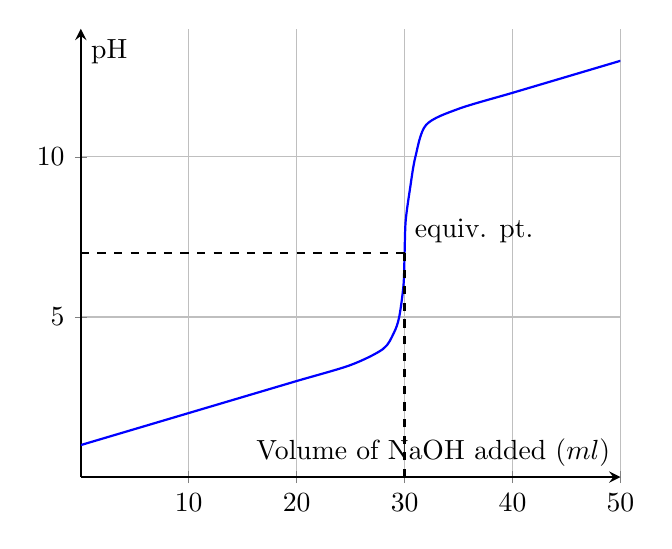
\begin{tikzpicture}
    \begin{axis}[
        xlabel={Volume of NaOH added ($ml$)},
        ylabel={pH},
        xmin=0, xmax=50,
        ymin=0, ymax=14,
        samples=100,
        thick,
        domain=0:50,
        grid=major,
        axis lines=middle
    ]
    % Titration curve for strong acid-strong base
    \addplot[blue, smooth] 
    coordinates {
        (0,1) (5,1.5) (10,2) (15,2.5) (20,3) (25,3.5) (28,4) 
        (29,4.5) (29.5,5) (29.9,6) (30,7) (30.1,8) (30.5,9) (31,10)
        (32,11) (35,11.5) (40,12) (45,12.5) (50,13)
    };
    
    % Mark equivalence point
    \draw[dashed] (0,7) -- (30,7) node[above right] {equiv. pt.};
    \draw[dashed] (30, 0) -- (30, 7);
    
    \end{axis}
\end{tikzpicture}
\end{center}

When performing a titration, try to aim for a light pink color. The \textbf{equivalence point} of a monobase/monoprotic acid is at pH = 7. For dibases/diprotic acids, there are 2 equivalence points, and the pH at these points varies.

\subsubsection{Titration Stoichiometry}
You use \textcolor{blue}{0.5 $M$ NaOH} to titrate a monoprotic acid. It takes \textcolor{blue}{15 $ml$ NaOH} to reach the equivalence point, and you started with \textcolor{blue}{25 $ml$} of acid. What is the acid concentration?

\textcolor{blue}{\textbf{Step 1:} Write and balance} the chemical formula.

$$\text{NaOH} + \text{HCl} \longrightarrow \text{H$_2$O} + \text{NaCl}$$

\textcolor{blue}{\textbf{Step 2:} Calculate the number of moles} of acid that you have.

$$(0.015 \: L \: \text{NaOH}) \times \left(\frac{0.5 \: mol \: \text{NaOH}}{1 \: L \: \text{NaOH}}\right) \times \left(\frac{1 \: mol \: \text{HCl}}{1 \: mol \: \text{NaOH}}\right) $$
$$=0.0075 \: mol \: \text{HCl}$$

\textcolor{blue}{\textbf{Step 3:} Put this number over the number of liters of acid you started with} to find the concentration (molarity).

$$\frac{0.0075 \: mol \: \text{HCl}}{0.025 \: L} = \boxed{0.3 \: M \: \text{HCl}}$$

\section{Serial Dilution}
A serial dilution is a series of multiple dilutions in a row.

\subsection{Dilution Steps}

\begin{enumerate}[leftmargin=*]
    \item Take 1 $ml$ of the original solution and add it to a second container.
    \item Add $x-1 \: ml$ of water.
    \item Repeat as many times as necessary. The molarity should have decreased by $x$ times (e.g. if you are performing a $1:4$ dilution and the original molarity was 1.0 $M$, the molarity after diluting once is 0.25 $M$).
\end{enumerate}

\subsection{Beer's Law}

\begin{equation}\label{beers}
A = \varepsilon l c
\end{equation}
where:
\begin{itemize}[leftmargin=*, nosep]
    \item $A$ is the absorbance
    \item $\varepsilon$ is the molar absorptivity (slope)
    \item $l$ is the pathlength
    \item $c$ is the concentration
\end{itemize}

\section{States of Matter}

\subsection{Three States of Matter}

\begin{table}[H]

\begin{tabular}{c|c|c|c}
\textbf{State of Matter} & \textbf{Conforms?} & \textbf{Closely packed?} & \textbf{Compressible?} \\\hline
solid & no & yes & no \\
liquid & yes & yes & no \\
gas & yes & no & yes
\end{tabular}

\vspace{1em}
Solids are not always more closely packed than liquids! There are exceptions, such as water.

\end{table}

\subsection{Temperature}
Kelvin K Fahrenheit \degF Celsius \degC

$$\degree \text{F} = 1.8(\degree\text{C}) + 32$$
$$\degree \text{C} = \frac{\degree \text{F} -32}{1.8}$$
$$\text{K} = \degree\text{C} + 273$$
$$\degree\text{C} = \text{K} - 273$$
$$\Delta T \: (\text{in} \degree\text{F}) = 1.8 \cdot \Delta T \: (\text{in} \degree\text{C or K})$$

\subsection{Kinetic Energy}
\begin{equation}\label{ke}
    \text{KE} = \frac{1}{2}mv^2
\end{equation}

Example: Which gas would move 4x faster than O$_2$?

Solution: Using \ref{ke}:

$$\frac{1}{2}(32 \: g/mol)(1 \: \text{(arbitrary unit of velocity))} = \frac{1}{2}(x \: g/mol)(4)$$
$$x = 2$$
$$\boxed{\text{H}_2}$$

\section{Gasses}

\subsection{Definitions}

\begin{itemize}[leftmargin=*, nosep]
    \item \textbf{\textit{gas pressure}}: Collisions of molecules with the container.
    \item \textbf{\textit{diffusion}}: The movement of particles from high concentration to low concentration until the concentration is consistent throughout.
    \item \textbf{\textit{effusion}}: The movement of particles through a small hole in the container.
    \item \textbf{\textit{long-range order}}: A regular, repetitive arrangement of particles. Solids with long-range order are called crystalline, and those without are called amorphous.
    \item \textbf{\textit{vapor pressure}}: Measure of the tendency of a liquid to vaporise.
\end{itemize}

\subsection{Pressure Units}
760 $mm$Hg (millimeters of mercury) = 1 $atm$ (atmosphere)

\subsection{The Gas Laws}
where:

\begin{itemize}[leftmargin=*, nosep]
    \item $P$ is the pressure
    \item $V$ is the volume
    \item $T$ is the temperature \textbf{in Kelvin}
    \item $n$ is the number of moles
    \item $R$ is the ideal gas constant equal to 0.0821
\end{itemize}

\begin{equation}\label{boyle}
    \text{\textbf{Boyle's Law: }}P_1V_1 = P_2V_2
\end{equation}
\begin{equation}\label{charles}
    \text{\textbf{Charles' Law: }}\frac{V_1}{T_1} = \frac{V_2}{T_2}
\end{equation}
\begin{equation}\label{gaylussac}
    \text{\textbf{Gay-Lussac's Law: }}\frac{P_1}{T_1} = \frac{P_2}{T_2}
\end{equation}
\begin{equation}\label{combined}
    \text{\textbf{Combined Gas Law: }}\frac{P_1V_1}{T_1} = \frac{P_2V_2}{T_2}
\end{equation}
\begin{equation}\label{avogadro}
    \text{\textbf{Avogadro's Law: }}\frac{V_1}{n_1} = \frac{V_2}{n_2}
\end{equation}
\begin{equation}\label{ideal}
    \text{\textbf{Ideal Gas Law: }}PV = nRT
\end{equation}

\paragraph{Important:}

\begin{itemize}[leftmargin=*, nosep]
    \item $P \propto T$ and $V \propto T$. $P \propto \frac{1}{V}$. (P and V are directly proportional to T, and P is proportional to the reciprocal of V or inversely proportional to V.)
    \item Always use K for temperature.
    \item Laws \ref{boyle}, \ref{charles}, and \ref{gaylussac} are only true \textbf{if the temperature, pressure, and volume are held constant.}
    \item The ideal gas law uses specific units. The constant $R$, 0.0821, uses the units $\frac{L \cdot atm}{mol \cdot \text{K}}$, so volume must be in $L$, pressure in $atm$, and, as always, temperature in K.
    \item STP (standard temperature and pressure) is at 0\degC or 273K when 1 $mol$ of any gas occupies 22.4 $l$.
\end{itemize}

Example: The density of an unknown gas at 20\degC and 749 $mm$Hg is 1.31 $g/L$. Calculate the molar mass of the gas.

Solution: Using \ref{ideal}, assuming 1 $L$ of the gas, and converting to proper units:

$$(0.986 \: atm)(1 \: L) = \R (293\text{K})(n)$$
$$n = 0.041 \: mol$$
$$1.31 \: g \div 0.041 \: mol$$
$$=\boxed{32.0 \: g/mol}$$

\subsection{Diffusion and Effusion}

\subsubsection{Law of Effusion}

\begin{equation}\label{effusion}
    \frac{\text{rate}_A}{\text{rate}_B} = \sqrt{\frac{\text{MM}_B}{\text{MM}_A}}
\end{equation}

where MM denotes molar mass.

Example: How many times faster does He effuse than N$_2$?

Solution: Using \ref{effusion}:

$$\frac{\text{rate}_\text{He}}{\text{rate}_\text{N$_2$}} = \sqrt{\frac{28.014}{4.003}}$$
$$=\boxed{2.65}$$

Example: Which gas diffuses 2.23 times faster than Br$_2$?

$$2.23 = \sqrt{\frac{159.808 \: g/mol}{x}}$$
$$x \approx 32 \: g/mol$$
$$\boxed{\text{O}_2}$$

\subsubsection{Other Formulas}

\begin{equation}\label{totalpressure}
    \text{\textbf{Total pressure: }} P_{\text{total}} = P_A + P_B + P_C + \cdots
\end{equation}
The total pressure of a mixture of gasses is equal to the sum of the pressures of its constituent parts.

\begin{equation}\label{molefraction}
    \text{\textbf{Definition of the mole fraction: }} \chi_a = \frac{n_A}{n_\text{total}}
\end{equation}
The mole fraction is defined as the number of moles of a substance over the moles of total gas.

\begin{equation}\label{partialpressure}
    \text{\textbf{Dalton's Law of Partial Pressure: }} P_a = \chi_a \cdot P_{\text{total}} 
\end{equation}
The pressure exerted by an individual gas is equal to the mole fraction times the total pressure.

Example: If you have 2.1 $mol$ N$_2$, 0.8 $mol$ CO$_2$, and 0.3 $mol$ O$_2$ at 297K and occupying 1.8 $L$, what is $P_{\text{total}}$ and the partial pressures?

\textcolor{blue}{\textbf{Step 1:} Add the number of moles together.}

$$2.1 + 0.8 + 0.3 = 3.2 \: mol$$

\textcolor{blue}{\textbf{Step 2:} Use $PV = nRT$} to find the total pressure.

$$PV = nRT$$
$$(1.8 \: L)(P) = \R (3.2 \: mol)(297\text{K})$$
$$P = 43.35 \: atm$$

\textcolor{blue}{\textbf{Step 3:} Find the mole fractions} for each element with \ref{molefraction}.

$$\chi_{\text{N}_2} = \frac{2.1 \: mol}{3.2 \: mol} = 0.656$$
$$\chi_{\text{CO}_2} = \frac{0.8 \: mol}{3.2 \: mol} = 0.25$$
$$\chi_{\text{O}_2} = \frac{0.3 \: mol}{3.2 \: mol} = 0.09$$

\textcolor{blue}{\textbf{Step 4:} Solve for partial pressure} with \ref{partialpressure}.

$$P_{\text{N}_2} = 0.656 \cdot 43.35 = 28.44 \: atm$$
$$P_{\text{CO}_2} = 0.25 \cdot 43.35 = 10.84 \: atm$$
$$P_{\text{CO}_2} = 0.09 \cdot 43.35 = 3.90 \: atm$$

$$\boxed{P_{\text{N}_2} = 28.44 \: atm; P_{\text{CO}_2} = 10.84 \: atm; P_{\text{O}_2} = 3.90 \: atm.}$$

\subsubsection{Phase Diagrams}
Below are the phase diagrams for typical material and water:\footnote{https://byjus.com/chemistry/phase-diagram-of-water/}

\begin{figure}[H]
\centering
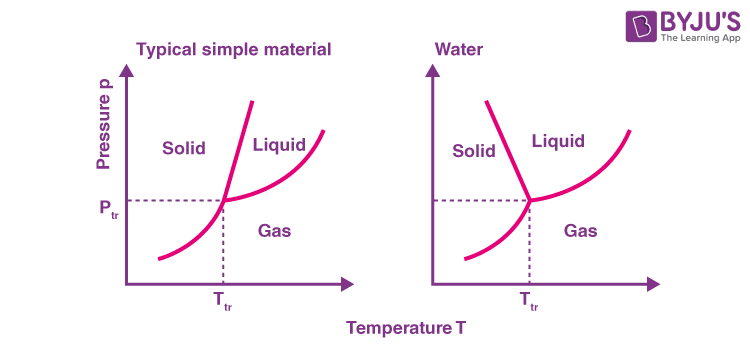
\includegraphics[width=0.7\textwidth]{phasediag.png}
\end{figure}

Note that in water, increasing the pressure leads to a phase change, since ice is less dense than water. The center point where all three lines intersect is called the \textbf{triple point}.

\subsubsection{Melting Points of Solids}
\textbf{Distinct melting point} (H$_2$O, metals...) v. \textbf{MP range} (fats, glass, plastic, rubber...)

Solids with distinct melting points are \textbf{crystalline} solids with long-range order. Solids with a melting point range are \textbf{amorphous} solids without long range order that melt at multiple temperatures.\footnote{https://elibraryportal.com/amorphous-and-crystalline-solids/}

\begin{figure}[H]
\centering
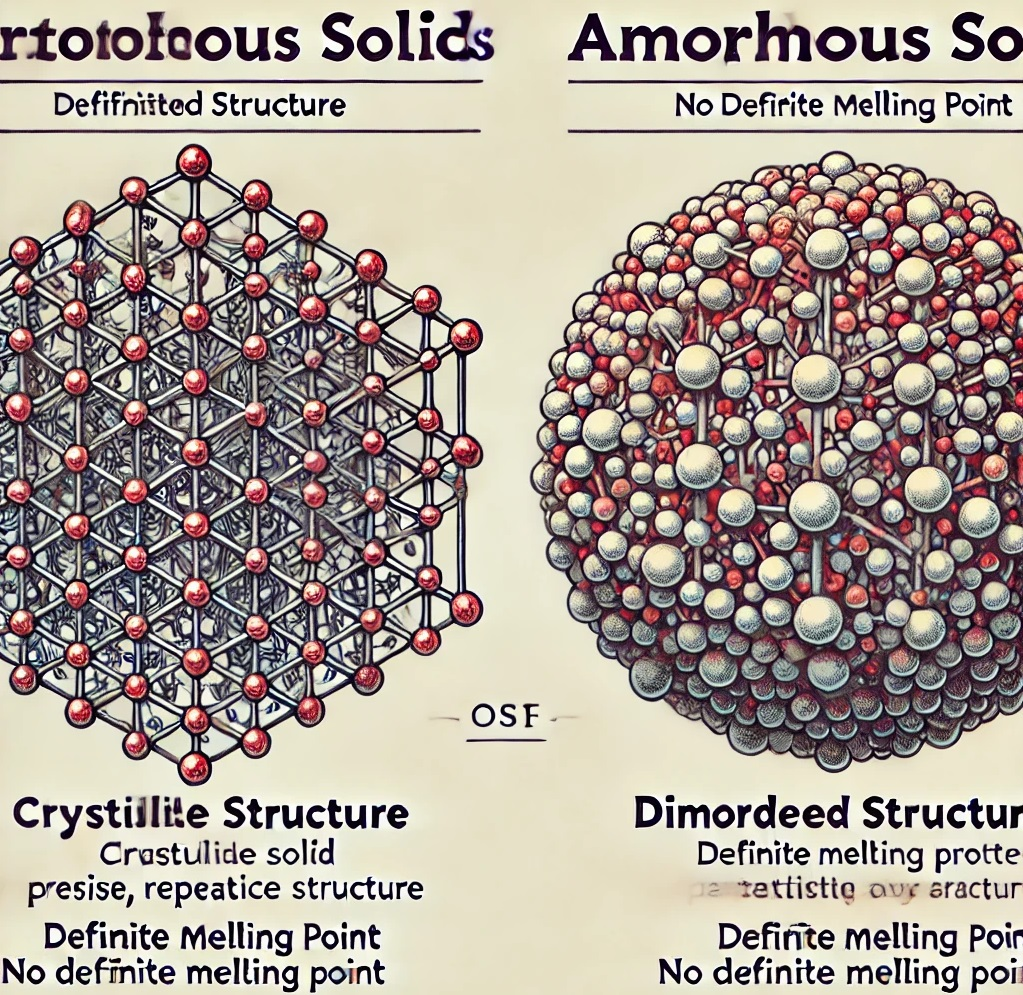
\includegraphics[width=0.5\textwidth]{funnypic.jpg}
\caption*{This is somewhat irrelevant, but here is an amusing AI-generated picture that attempts to explain this concept. (They tried.)}
\end{figure}

\subsubsection{Vapor Pressure}
As temperature increases, vapor pressure will also increase until vapor pressure is equal to the atmospheric pressure (i.e. the boiling point). There is an exchange of molecules happening at the surface of a liquid, and if you seal the container, it will eventually reach equilibrium.

\subsubsection{Solutions}
\textbf{Freezing point depression} happens when a non-volatile solute is added to a solvent that disrupts the lattice, interfering with the solvent's ability to form its regular crystalline structure.

\textbf{Boiling point elevation} happens when a non-volatile solute is added to a solvent and blocks the solvent from evaporating.

\section{Thermodynamics}
\subsection{Definitions}

\begin{itemize}[leftmargin=*, nosep]
\item \textbf{\textit{heat}}: The kinetic energy of particles.
\item \textbf{\textit{temperature}}: The measurement of heat.
\item \textbf{\textit{endothermic process}}: A process that absorbs heat from surroundings, going from a lower energy state to a higher energy state.
\item \textbf{\textit{exothermic process}}: A process that releases heat into surroundings, going from a higher energy state to a lower energy state.
\item \textbf{\textit{calorie}}: The amount of energy it takes to raise 1 gram of water by 1 degree Celsius (specific heat capacity of water).
\item \textbf{\textit{specific heat capacity}}: The amount of energy it takes to raise the temperature of 1 gram of a substance by 1 degree Celsius. (For water, the specific heat capacity is 1 calorie.)
\item \textbf{\textit{bond energy}}: The heat required to break a bond or released when the bond is made.
\end{itemize}

\subsection{Laws of Thermodynamics}

\begin{enumerate}[leftmargin=*, nosep]
\item \textbf{Energy cannot be created nor destroyed.}
\item \textbf{Heat disperses until equal.}
\end{enumerate}

\subsection{Reaction Diagrams for Chemical Changes}
Below are the reaction diagrams for endothermic and exothermic reactions:\footnote{https://online-learning-college.com/knowledge-hub/gcses/gcse-chemistry-help/energy-level-diagrams/}

\begin{figure}[H]
\centering
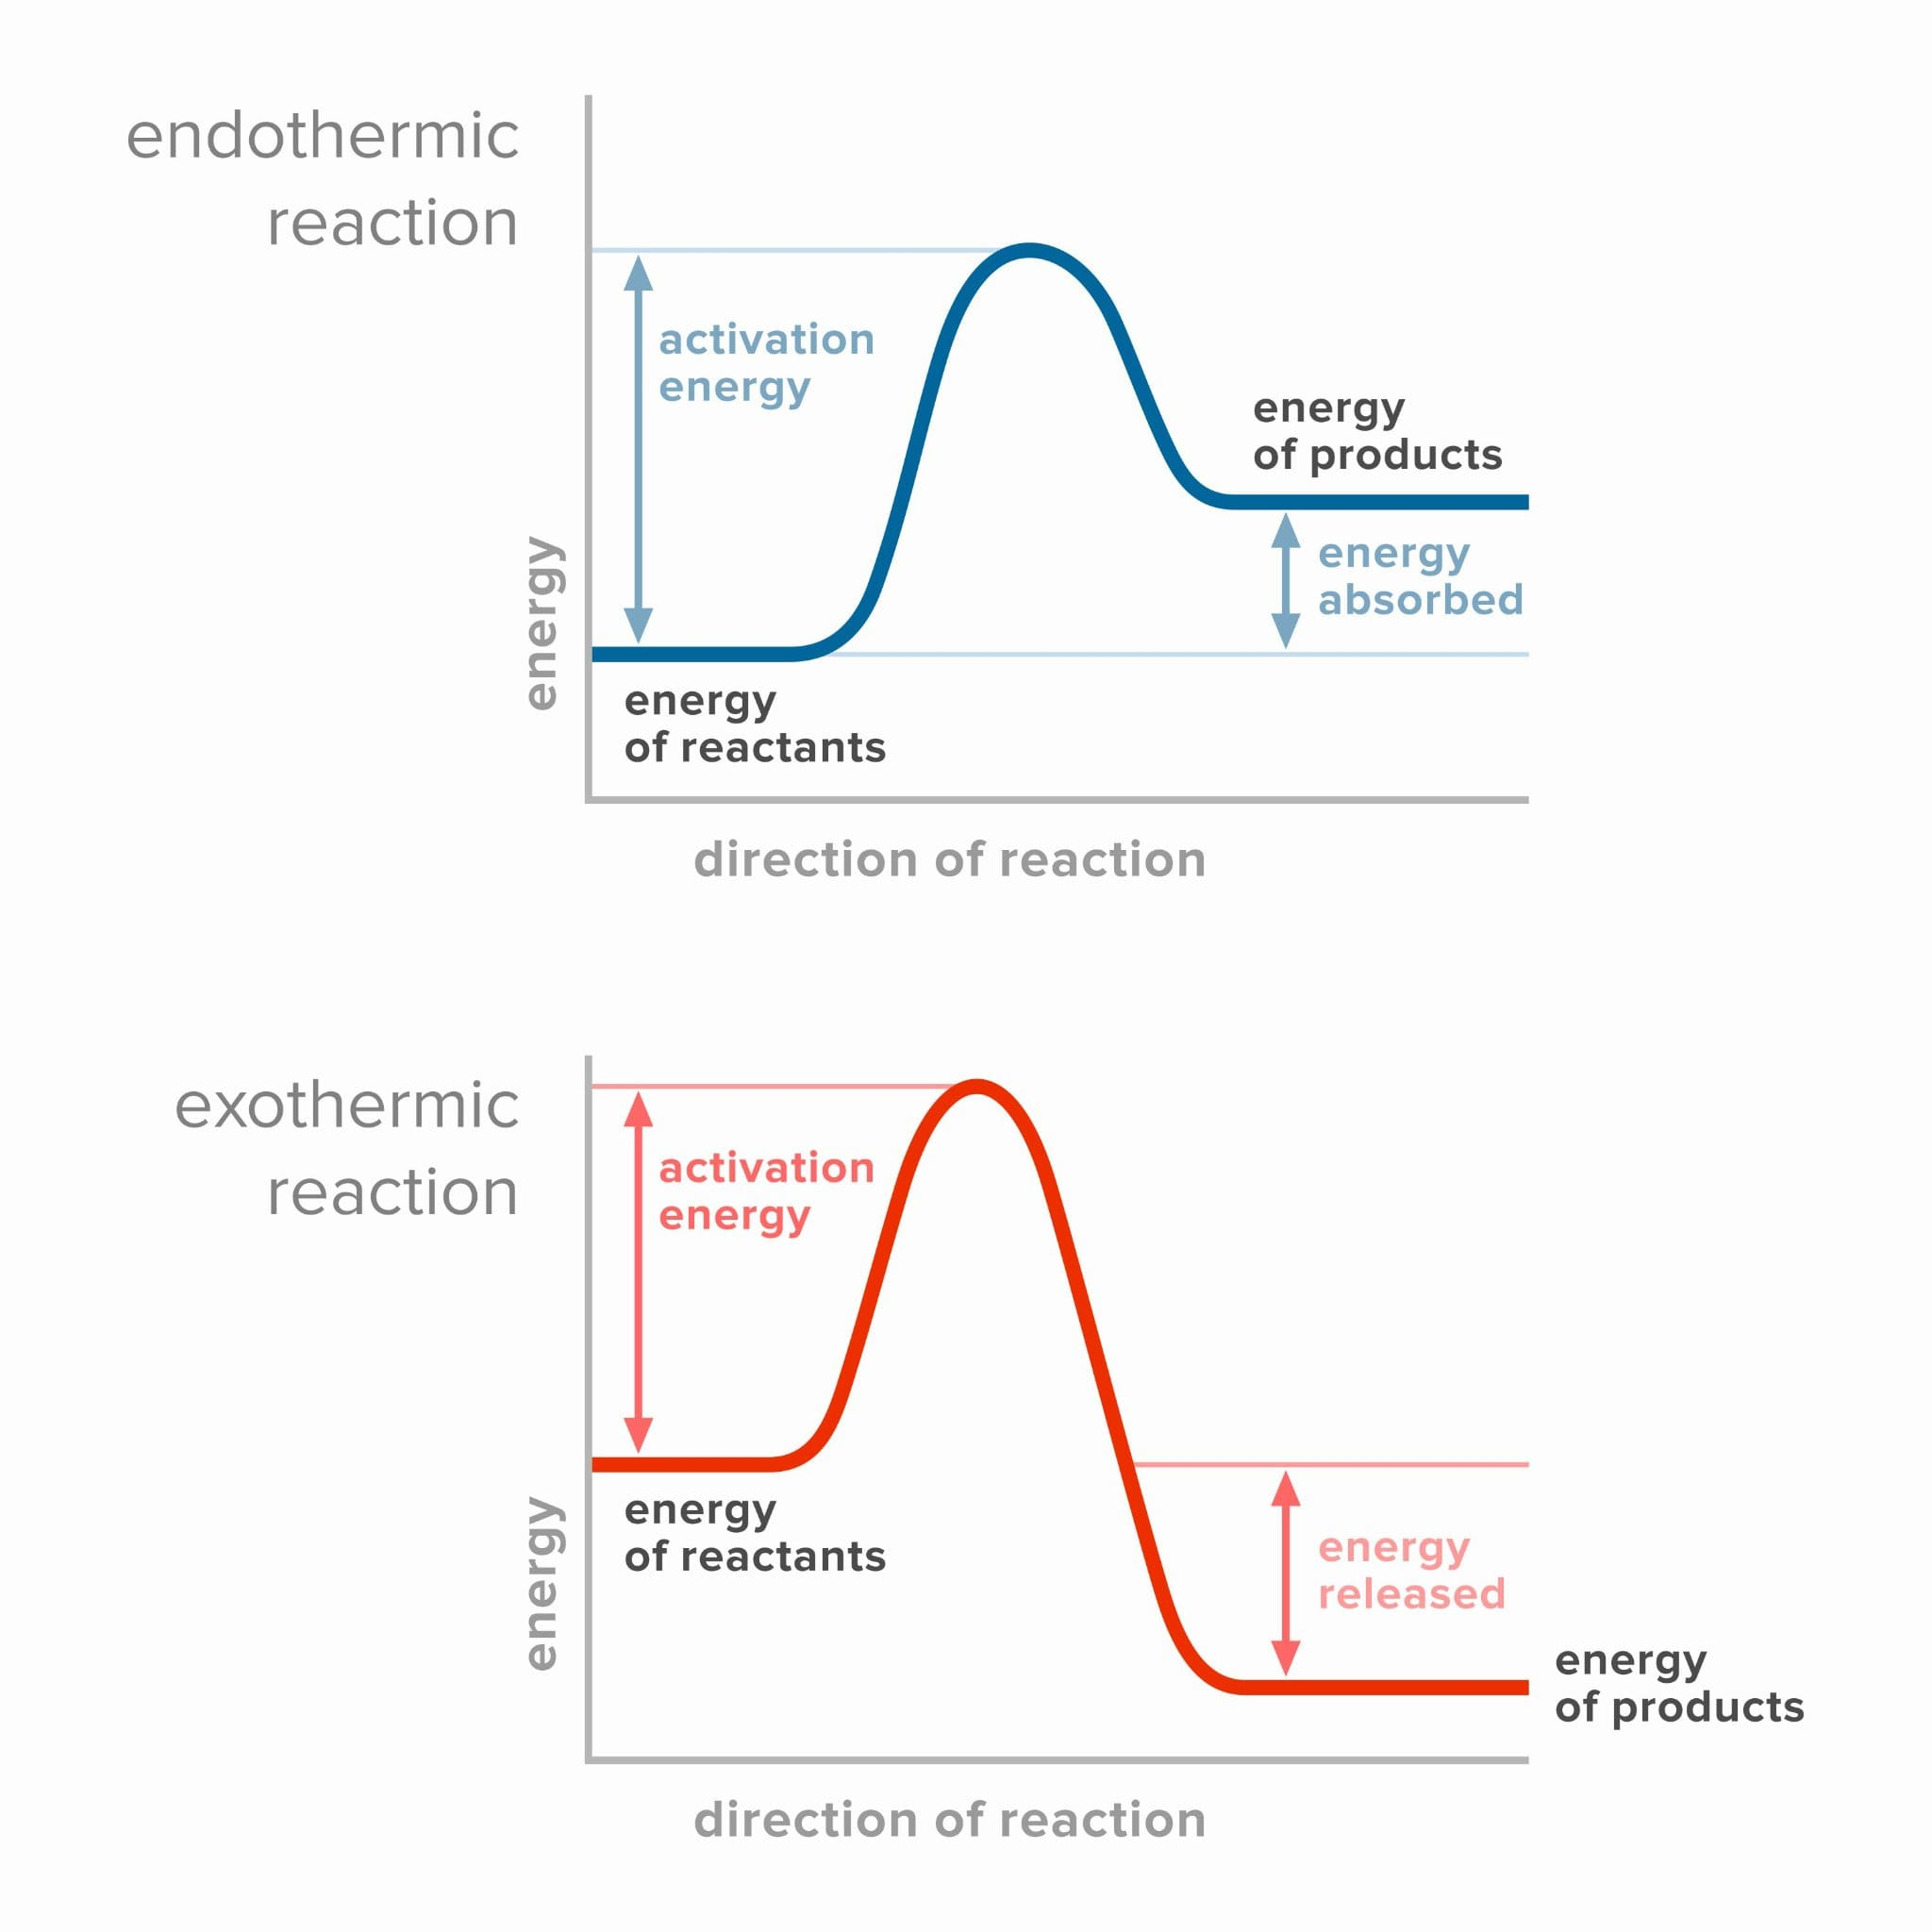
\includegraphics[width=0.6\textwidth]{eldiag.jpg}
\end{figure}

Activation energy, or \(E_a\), is the energy required to undergo a specific reaction. Energy released/absorbed is denoted by \(\Delta H\).

\subsection{Heat Transfer}

\begin{equation}\label{heattransfer}
q = mc \Delta T
\end{equation}
where:
\begin{itemize}[leftmargin=*, nosep]
\item $q$ is heat in joules
\item $m$ is mass in grams
\item $c$ is the specific heat capacity in joules over degrees Celsius
\item $\Delta T$ is the change in temperature in degrees Celsius or Kelvin
\end{itemize}

\subsubsection{Heat Units}

1 kilocalorie/food calorie (kcal or Cal) = 1000 calories (cal) = 4184 joules (J)

\subsection{Heat Curves}
A heat curve for water:\footnote{This is hand-drawn because I have not yet mastered the art of TikZ. Maybe soon?}

\begin{figure}[H]
\centering
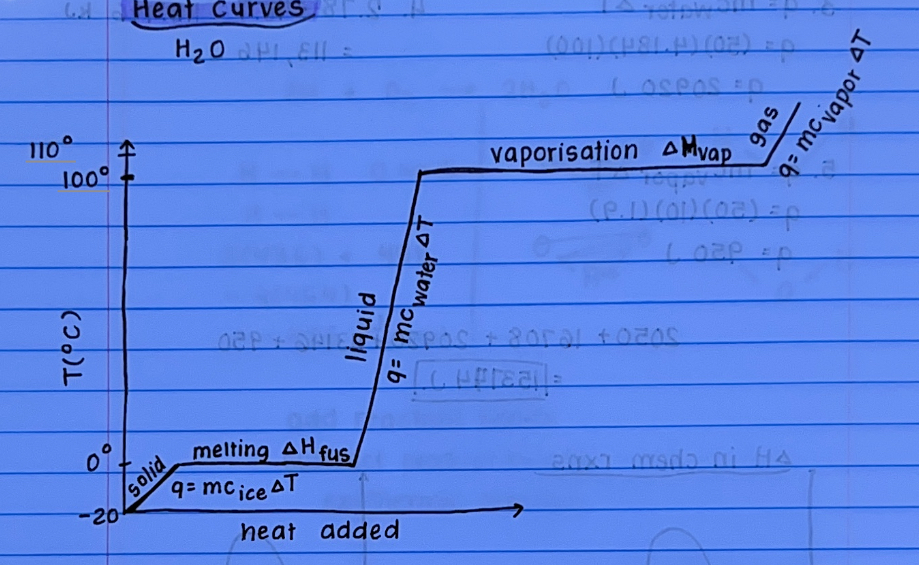
\includegraphics[width=0.7\textwidth]{heatcurve.jpg}
\end{figure}

$\Delta H_\text{fusion}$: amt of heat/mol that is absorbed when melting or released when freezing
$\Delta H_\text{vapor}$: amt of heat/mol absorbed when vaporising/released when condensing

Example: How much heat does it take to change 50 $g$ of water from a solid state at -20 \degC to a vapor state at 110 \degC?

Given:

\begin{itemize}[leftmargin=*, nosep]
	\item melting point of water: 0 \degC
	\item boiling point of water: 100 \degC
	\item $c_\text{ice}$ = 2.05 \cunits
	\item $c_\text{water}$ = 4.814 \cunits
	\item $c_\text{vapor}$ = 1.9 \cunits
	\item $\Delta H_\text{fus}$ = 6.01 $\frac{kJ}{mol}$
	\item $\Delta H_\text{vap}$ = 40.7 $\frac{kJ}{mol}$
\end{itemize}

This solution takes five steps. At the end, add them all together.

\textcolor{blue}{\textbf{Step 1:} Solid state.} The melting point of water is 0 \degC and the $\Delta T$ is 20. Use \(q = mc_\text{ice}\Delta T\):

\[q = (50)(2.05)(20) = 2050 \: J\]

\textcolor{blue}{\textbf{Step 2:} Fusion (melting).} By a simple calculation, we can find that there are 2.78 $mol$ of water. Convert to kilojoules, then to joules:

\[6.01 \: \frac{kJ}{mol} \cdot 2.78 \: mol = 16.708 \: kJ = 16708 \: J\]

\textcolor{blue}{\textbf{Step 3:} Liquid state.} The boiling point of water is 100 \degC and the $\Delta T$ is 100. Use \(q = mc_\text{water}\Delta T\):

\[q = (50)(4.184)(100) = 20920 \: J\]

\textcolor{blue}{\textbf{Step 2:} Vaporisation (boiling).} Using the same 2.78 $mol$ of water, convert $\Delta H_\text{vap}$ to kilojoules, then to joules:

\[40.7 \: \frac{kJ}{mol} \cdot 2.78 \: mol = 113.146 \: kJ = 113146 \: J\]

\textcolor{blue}{\textbf{Step 5:} Vapor state.} The final temperature is 110 \degC and the $\Delta T$ is 10. Use \(q = mc_\text{vapor}\Delta T\):

\[q = (50)(1.9)(10) = 950 \: J\]

\textcolor{blue}{\textbf{Step 6:} Add each change in heat together.}

\[2050 + 16708 + 20920 + 113146 + 950\]
\[=\boxed{153774 \: J}\]

\subsection{$\Delta H$ in Reactions}
Breaking bonds \textbf{absorbs} heat, and making bonds \textbf{releases} heat. A positive $\Delta H$ suggests an endothermic reaction, and a negative $\Delta H$ suggests an exothermic reaction. To find the $\Delta H$ from a chemical equation, subtract the bond energies of the products from those of the reactants.

\subsection{Hess' Law}
When adding reactions, you can also add $\Delta H$ values.

Example: Find the $\Delta H$ of the overall reaction.

$$\text{Overall rxn}: \text{CH}_{4(g)} + \text{H$_2$O}_{(g)} \longrightarrow \text{CO}_{(g)} + \text{3H}_{2(g)}$$
$$\text{CO}_{(g)} + \nicefrac12 \text{O}_{2(g)} \longrightarrow \text{CO}_{2(g)}, \Delta H = -283 \: \frac{kJ}{mol}$$
$$\text{H}_{2(g)} + \nicefrac12 \text{O}_{2(g)} \longrightarrow \text{H$_2$O}_{(g)}, \Delta H = -242 \: \frac{kJ}{mol}$$
$$\text{CH}_{4(g)} + \text{2O}_{2(g)} \longrightarrow \text{CO}_{2(g)} + \text{2H$_2$O}_{(g)}, \Delta H = -803 \: \frac{kJ}{mol}$$

Manipulate the three equations so that all the unnecessary elements cancel out:

$$\text{Flip}: \cancel{\text{CO}_{2(g)}} \longrightarrow \text{CO}_{(g)} + \cancel{\nicefrac12 \text{O}_{2(g)}}, \Delta H = 283 \: \frac{kJ}{mol}$$
$$\text{Flip and multiply by 3}: \cancel{\text{3H$_2$O}_{(g)}} \text{H$_2$O}_{(g)} \longrightarrow \text{3H}_{2(g)} + \cancel{\nicefrac32 \text{O}_{2(g)}}, \Delta H = 726 \: \frac{kJ}{mol}$$
$$\text{Leave as is}: \text{CH}_{4(g)} + \cancel{\text{2O}_{2(g)}} \longrightarrow \cancel{\text{CO}_{2(g)}} + \cancel{\text{2H$_2$O}_{(g)}}, \Delta H = -803 \: \frac{kJ}{mol}$$

Leaving us with the overall reaction:

$$\text{CH}_{4(g)} + \text{H$_2$O}_{(g)} \longrightarrow \text{CO}_{(g)} + \text{3H}_{2(g)}$$

Adding the $\Delta H$ values:

$$283 + 726 - 803$$
$$ = \boxed{206 \: \frac{kJ}{mol}.}$$

\section{Gasses and Heat in Stoichiometry}

\subsection{Heat of Reaction Stoichiometry}
$$7\text{H}_{2(g)} + 2\text{NO}_{2(g)} \longrightarrow 2\text{NH}_{3(g)} + 4\text{H$_2$O}_{(l)} \quad \Delta H = 142.5 \: kJ$$

In the above equation, what would $\Delta H$ be if 4.8 $mol$ of H$_2$ were reacted? Is this reaction endothermic or exothermic? Where does heat belong in this equation: with the reactants or products?

This reaction is \textbf{endothermic} because the $\Delta H$ is positive, meaning it absorbs heat. Heat belongs on the \textbf{reactants} side.

$$7\text{H}_{2(g)} + 2\text{NO}_{2(g)} + \text{heat} \longrightarrow 2\text{NH}_{3(g)} + 4\text{H$_2$O}_{(l)} \quad \Delta H = 142.5 \: kJ$$

\textcolor{blue}{\textbf{Step 1:} Find the heat per mole} of H$_2$.

$$\frac{142.5 \: kJ}{7 \: mol \: \text{H}_2} = 20.36 \: \frac{kJ}{mol}$$

\textcolor{blue}{\textbf{Step 2:} Find the total heat} by multiplying by 4.8 $mol$.

$$20.36 \: \frac{kJ}{mol} \times 4.8 \: mol = \boxed{97.73 \: kJ}$$

If 4.8 $mol$ of H$_2$ were reacted, the $\Delta H$ would be 97.73 $kJ$.

\subsection{Gasses}
$$6 \text{HCl} + 2 \text{Al} \longrightarrow 2 \text{AlCl}_3 + 3\text{H}_2$$

At STP, how many $ml$ of H$_2$ gas are produced from 12 $g$ of solid Al? (1 $mol$ = 22.4 $L$ at STP)

Using stoichiometry:

$$(12 \: g \: \text{Al}) \times \left(\frac{1 \: mol \: \text{Al}}{26.98 \: g \: \text{Al}}\right) \times \left(\frac{3 \: mol \: \text{H}_2}{2 \: mol \: \text{Al}}\right) \times \left(\frac{22.4 \: L \: \text{H}_2}{1 \: mol \: \text{H}_2}\right) \times \left(\frac{1000 \: ml}{1 \: L}\right)$$
$$ = \boxed{14944.4 \: ml}$$

\subsection{Heats of Formation}
\Hf{} is the heat absorbed/released when compounds are formed from elemental units. The \Hf{} of elements, including diatomic elements, is always 0.

Heats of formation equation:

\begin{equation} \label{heatsofform}
\Delta H_\text{rxn} = \sum \Delta H_\text{f(products)} -  \sum \Delta H_\text{f(reactants)}
\end{equation}

$$\text{CS}_2 + 3\text{O}_2 \longrightarrow \text{CO}_2 + 2\text{SO}_2$$

Find the heat of formation given the following: 

$$\mathHf \: (\text{CO}_2) = -393.5 \: \frac{kJ}{mol}$$
$$\mathHf \: (\text{SO}_2) = -296.8 \: \frac{kJ}{mol}$$
$$\mathHf \: (\text{CS}_2) = 87.9 \: \frac{kJ}{mol}$$

Solution: Using \ref{heatsofform}:

$$ [-393.5 + 2(-296.8)] - [3(0) + 87.9] $$
$$ = \boxed{1075 \: \frac{kJ}{mol}} $$

\section{Redox}

\subsection{Definitions}

\begin{itemize}[leftmargin=*, nosep]
\item \textbf{\textit{redox reaction}}: Short for \textit{oxidation/reduction reaction}.
\item \textbf{\textit{oxidation}}: Losing electrons (becoming more positive). 
\item \textbf{\textit{reduction}}: Gaining electrons (becoming more negative).
\item \textbf{\textit{oxidizing agent}}: Oxidizing another compound and is being reduced.
\item \textbf{\textit{reducing agent}}: Reducing another compound and is being oxidized.
\end{itemize}

\subsection{Reactions}
LEO the lion says GER (Losing Electrons = Oxidation, Gaining Electrons = Reduction)

\begin{align*}
\text{Na} \longrightarrow \text{Na}^+ + e^- \hspace{2em} & \text{oxidation \nicefrac12 reaction} \\
\text{Cl}_2 + 2e^- \longrightarrow 2\text{Cl}^- \hspace{2em} & \text{reduction \nicefrac12 reaction} \\
2\text{Na} + \text{Cl}_2 \longrightarrow 2\text{NaCl} \hspace{2em} & \text{overall reaction}
\end{align*}

\subsection{Assigning Oxidation Numbers}

\subsubsection{Rules}
\begin{enumerate}
\item An element in its elemental state is neutral.
\item H in a compound is always +1.
\item O in a compound is -2 except for H$_2$O$_2$; in that case, the oxidation number of O is -1.
\item Monatomic ions are whatever ionic charge they would normally form.
\item All oxidation numbers must add to the overall charge of the molecule or ion.
\end{enumerate}

Example: What is the oxidation number of I in Mg(IO$_3$)$_2$?

Solution: By looking at the charge on Mg, the charge on (IO$_3$)$_2$ can be found to be 2-, so the charge on one ion is 1-, making the ion (IO$_3$)$^-$. The oxidation number of O in this compound is 2- by rule 3. There are 3 oxygen atoms, so:

$$3(-2) + \text{I} = -1$$

Solving for I:

$$-6 + \text{I} = -1$$
$$\text{I} = -1+6$$
$$\text{I} = 5$$

The charge on I is \fbox{+5}.

\subsection{Writing Half-Reactions}
$$2\text{Ag} + \text{H}_2\text{S} \longrightarrow \text{Ag}_2\text{S} + \text{H}_2$$

To write half-reactions, look at the oxidation numbers on each element. If the oxidation number has increased, it has been oxidised. If the number has decreased, it has been reduced.

Oxidation \nicefrac12 reaction:
$$2\text{Ag} \longrightarrow  \text{(break the ionic bond)} \: 2\text{Ag}^+ + 2e^-$$

Reduction \nicefrac12 reaction:
$$2\text{H}^+ + 2e^- \longrightarrow \text{H}_2$$

If \textit{none} of the oxidation numbers change, the reaction is \textit{not} a redox reaction. For example,

$$\text{Al}_2\text{S}_3 + 6 \text{H}_2\text{O} \longrightarrow 2\text{Al(OH)}_3 + 3\text{H}_2\text{S}$$

is not a redox reaction.

\subsection{Balancing Redox Reactions}
Assume an acidic, aqueous environment:

$$\text{PbO}_2 + \text{I}_2 \longrightarrow \text{Pb}^{2+} + \text{IO}_3^-$$

\begin{enumerate}[leftmargin=*]
\item Separate into oxidation and reduction half-reactions by looking at oxidation numbers.

\begin{gather*}
\text{Oxidation half-reaction:} \: \text{I}_2 \longrightarrow \text{IO}_3^- \\
\text{Reduction half-reaction:} \: \text{PbO}_2 \longrightarrow \text{Pb}^{2+}
\end{gather*}

\item Balance elements that are \textit{not} H or O.

\begin{gather*}
\text{I}_2 \longrightarrow 2\text{IO}_3^- \\
\text{PbO}_2 \longrightarrow \text{Pb}^{2+}
\end{gather*}

\item Balance O by adding H$_2$O.

\begin{gather*}
6\text{H$_2$O} + \text{I}_2 \longrightarrow 2\text{IO}_3^- \\
\text{PbO}_2 \longrightarrow \text{Pb}^{2+} + 2\text{H$_2$O}
\end{gather*}

\item Balance H by adding H$^+$.

\begin{gather*}
6\text{H$_2$O} + \text{I}_2 \longrightarrow 2\text{IO}_3^- + 12\text{H}^+\\
4\text{H}^+ + \text{PbO}_2 \longrightarrow \text{Pb}^{2+} + 2\text{H$_2$O}
\end{gather*}

\item Add electrons to balance the charges. When balanced correctly, electrons should be on opposite sides (one on reactants, one on products). 

\begin{gather*}
6\text{H$_2$O} + \text{I}_2 \longrightarrow 2\text{IO}_3^- + 12\text{H}^+ + 10e^-\\
2e^- + 4\text{H}^+ + \text{PbO}_2 \longrightarrow \text{Pb}^{2+} + 2\text{H$_2$O}
\end{gather*}

\item Multiply to cancel out the electrons.

\begin{gather*}
6\text{H$_2$O} + \text{I}_2 \longrightarrow 2\text{IO}_3^- + 12\text{H}^+ + 10e^-\\
10e^- + 20\text{H}^+ + 5\text{PbO}_2 \longrightarrow 5\text{Pb}^{2+} + 10\text{H$_2$O}
\end{gather*}

\item Combine and cancel.

\begin{gather*}
\cancel{6\text{H$_2$O}} + \text{I}_2 \longrightarrow 2\text{IO}_3^- + \cancel{12\text{H}^+} + \cancel{10e^-}\\
\cancel{10e^-} + \cancel{20\text{H}^+} 8\text{H}^+ + 5\text{PbO}_2 \longrightarrow 5\text{Pb}^{2+} + \cancel{10\text{H$_2$O}} 4\text{H$_2$O} \\
\boxed{\text{I}_2 + 8\text{H}^+ + 5\text{PbO}_2 \longrightarrow 5\text{Pb}^{2+} + 4\text{H$_2$O} + 2\text{IO}_3^-}
\end{gather*}

\end{enumerate}

\section{Batteries}
Below is a diagram of a Voltaic/Galvanic cell\footnote{bit.ly/4jMzl6a}:
\begin{figure}[H]
\centering
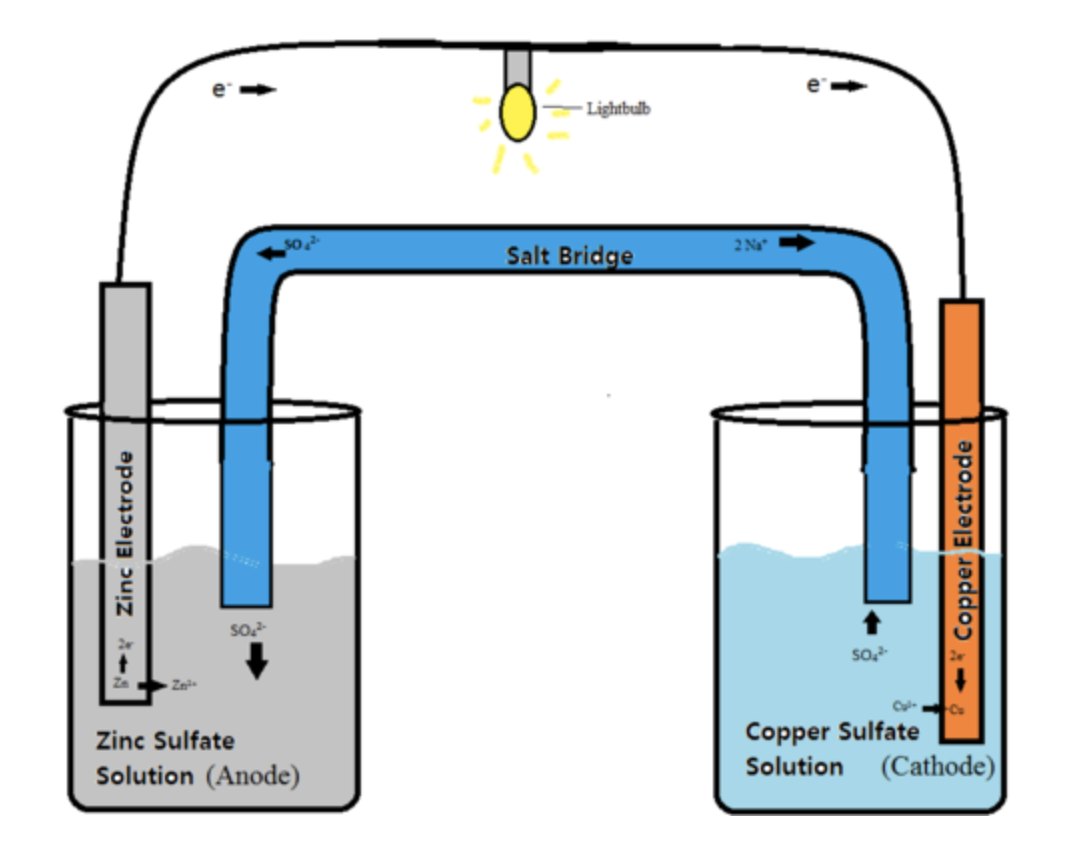
\includegraphics[width=0.6\textwidth]{voltaiccell}
\end{figure}

containing:

\begin{description}
\item[electrodes] to carry electricity. The \textbf{anode} is oxidised, losing mass as the material is released into solution, and the \textbf{cathode} is reduced, gaining mass as solid metal deposits onto it.
\item[salt bridge] to close the circuit. 
\item[solutions] that the electrodes are suspended in. 
\end{description}

Electrons flow from the anode to the cathode.

To find the voltage of this battery:

$$\text{Cu}^{2+} + 2e^- \longrightarrow \text{Cu} \: (0.34 \: \text{V})$$
$$\text{Zn}^{2+} + 2e^- \longrightarrow \text{Zn} \: (-0.726 \: \text{V})$$

Flip the equation that is higher on the standard reduction potential table:

$$\text{Cu}^{2+} + 2e^- \longrightarrow \text{Cu} \: (0.34 \: \text{V, reduction reaction})$$
$$\text{Zn} \longrightarrow \text{Zn}^{2+} + 2e^- \: (0.726 \: \text{V, oxidation reaction})$$

Combine:

$$\text{Cu}^{2+} + \text{Zn} \longrightarrow \text{Cu} + \text{Zn}^{2+} \: \boxed{(1.1 \: \text{V})}$$

\textsc{n.b.} When \textbf{multiplying} an equation to balance out the electrons, \textbf{the voltage does not change.} It only changes in sign if the equation is flipped.

\section{Nuclear Chemistry}

\subsection{Types of Radioactive Decay}
\textbf{Radioactive decay}, or \textbf{nuclear radiation}, is the release of particles/energy from unstable nuclei (radio isotopes).

There are three types:

\begin{description}
\item [$\alpha$-radiation] \ce{^{4}_{2}He} released, penetrates $\sim \frac{1}{20} \: mm$ into body tissue, blocked by paper
\item [$\beta$-radiation] \ce{^{0}_{-1}$e$} released, penetrates $\sim 4 \: mm$ into body tissue, blocked by aluminum foil
\item [$\gamma$-radiation] \ce{^{0}_{0}$\gamma$} released, penetrates several inches of lead and feet of concrete
\end{description}

\subsection{Half-lives}
The half-life of a radioisotope sample is the amount of time it takes for 50\% of it to decay. Each sample has its own distinct half-life. The amount of sample left follows an exponential decay model that reaches 0 asymptotically.

The half-life formula is:

\begin{equation}\label{eq:halflife}
N = N_0 \left(\frac{1}{2}\right)^{\frac{t}{t_{1/2}}}
\end{equation}

where:

\begin{itemize}[leftmargin=*, nosep]
\item $N$ = final amount of sample
\item $N_0$ = initial amount of sample
\item $t$ = time elapsed
\item $t_{1/2}$ = half-life
\end{itemize}

\end{document}